\documentclass[t,aspectratio=169,usenames,dvipsnames,xcolor=table]{beamer}
\usepackage{redhat-beamer/redhat}
\usepackage{layout}
\usepackage{xcolor}
\usepackage{ulem}
\usepackage{pifont}
\usepackage{makecell}

\definecolor{hlcolor}{RGB}{2,65,77}
\definecolor{bgcolor}{RGB}{241,241,241}
\definecolor{rhreddark}{RGB}{163,0,0}

\newcommand{\hll}[1]{{\color{rhred} #1}}
\newcommand{\hl}[1]{\textbf{\hll{#1}}}

%
% font
%
\usepackage{fontspec}
\usepackage{fontawesome}
\setmonofont{FreeMono}

\usepackage{tikz}
\usetikzlibrary{positioning,calc}

\usepackage{listings}
\usepackage{lstautogobble}
\lstset{
    language=C,
    basicstyle={\tiny\ttfamily},
    autogobble=true,
    moredelim=**[is][\only<1>{\color{rhred}\bfseries}]{^}{^},
    moredelim=**[is][\only<2->{\color{rhred}\bfseries}]{@}{@},
    moredelim=**[is][\only<2->{\color{blue}\bfseries}]{~}{~},
}

\renewcommand<>{\sout}[1]{
  \alt#2{\beameroriginal{\sout}{#1}}{#1}
}

\tikzset{onslide/.code args={<#1>#2}{%
  \only<#1>{\pgfkeysalso{#2}} % \pgfkeysalso doesn't change the path
}}

\title{Advanced Git}
\subtitle{IVS demonstration exercise}
\author{Viktor Malík \and Petr Stodůlka \and Pavel Odvody}
\institute{Red Hat}
\date{March 31, 2023}

\begin{document}

\maketitle

\begin{frame}
  \frametitle{Prerequisites}
  \vspace{-1.5em}
  \begin{itemize}
    \setlength\itemsep{1em}
    \item Basic knowledge of Git commands for:
      \begin{itemize}
      \setlength\itemsep{.3em}
        \item creating commits (\texttt{git add, git commit})
        \item inspecting current state (\texttt{git status, git diff})
        \item inspecting history (\texttt{git log, git show})
        \item working with remotes (\texttt{git pull, git push})
        \item working with branches (\texttt{git checkout, git branch})
        \item merging branches (\texttt{git merge, git rebase})
      \end{itemize}
    \item Git commands cheatsheet:\\
      \footnotesize\url{https://www.atlassian.com/git/tutorials/atlassian-git-cheatsheet}
  \end{itemize}
\end{frame}

\begin{frame}
  \frametitle{Git cherry pick}
  \begin{itemize}
    \vspace{-1.5em}
    \item \texttt{git cherry-pick} allows to \textbf{copy} a commit from one
      branch to another
  \end{itemize}

  \vspace{1em}
  \begin{columns}[c]
    \begin{column}{.5\textwidth}
      \centering
      \onslide*<1>{
        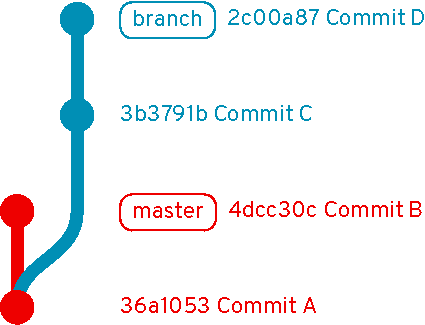
\includegraphics[scale=0.6]{git-figures/cherry-pick-pre.pdf}\\[1em]
      }
      \onslide*<2->{
        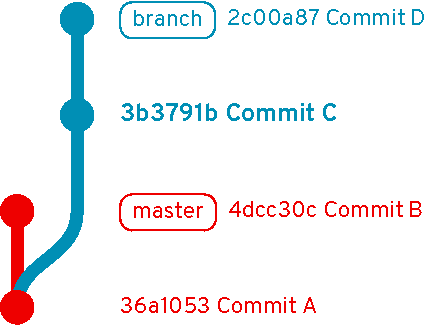
\includegraphics[scale=0.6]{git-figures/cherry-pick-pre-highlight.pdf}\\[1em]
      }
      \onslide<2->{
        \hspace{2em}\texttt{git cherry-pick 3b3791b}
      }
    \end{column}
    \onslide<3>{
    \begin{column}{.5\textwidth}
      \centering
      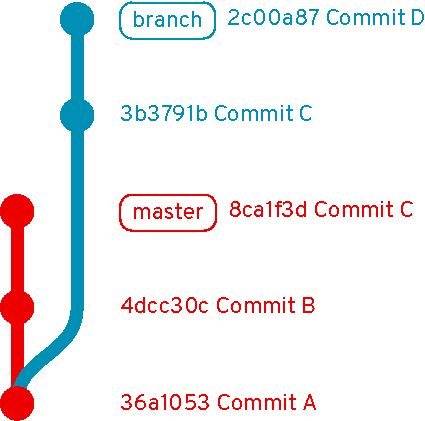
\includegraphics[scale=0.6]{git-figures/cherry-pick-post.pdf}
    \end{column}
    }
  \end{columns}
\end{frame}

\begin{frame}
  \frametitle{Git commit ranges}
  \begin{columns}[c]
    \begin{column}{.7\textwidth}
      \begin{itemize}
      \setlength\itemsep{.8em}
        \item<1-> \texttt{2756e30..af94919} selects all commits from
          \textit{Commit~D} (inclusive) to \textit{Commit~B} (exclusive)
        \item<2-> \texttt{af94919\textasciicircum} gives the parent of
          \textit{Commit~B} (\textit{Commit~A})
        \item<3-> Hence, \texttt{2756e30..af94919\textasciicircum} selects
          the commit range including \textit{Commit~B}
        \item<4> \textbf{Note:} the order of references does not matter.\\
          \texttt{2756e30..af94919\textasciicircum} =
          \texttt{af94919\textasciicircum..2756e30}
      \end{itemize}
    \end{column}
    \begin{column}{.3\textwidth}
      \begin{tikzpicture}
        \node at (0,0) {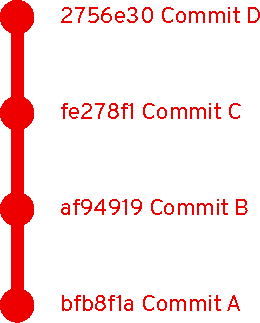
\includegraphics[scale=0.6]{git-figures/commit-ranges.pdf}};
        \onslide<1>{
          \draw (-1.7,0) rectangle ++(4,2) {};
        }
        \onslide<2>{
          \draw (-1.7,-2) rectangle ++(4,1) {};
        }
        \onslide<3->{
          \draw (-1.7,-1) rectangle ++(4,3) {};
        }
      \end{tikzpicture}
    \end{column}
  \end{columns}
\end{frame}

\section{''Advanced'' work with Git}

\begin{frame}
  \frametitle{Let's start}
  \begin{itemize}
    \setlength\itemsep{.5em}
    \item We'll write a simple tool for counting characters, words, and lines
      in a file (similar to the \texttt{wc} utility)
    \item We start with a pre-initialized repo containing very basics of the
      tool:\\
      \url{https://github.com/viktormalik/git-workshop}
    \item The repo contains:
      \begin{itemize}
        \item source file \texttt{wc.c}
        \item testing file \texttt{testfile}
        \item \texttt{Makefile}
        \item \texttt{.gitignore}
      \end{itemize}
  \end{itemize}
\end{frame}

\begin{frame}
  \frametitle{Current status of the repo}
  \centering
  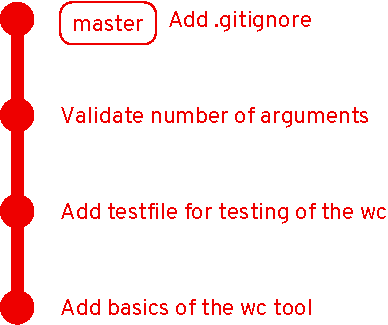
\includegraphics[scale=0.8]{git-figures/01-initial.pdf}
\end{frame}

\begin{frame}
  \frametitle{Basic team synchronisation}
  \vspace{-1em}
  Every member implements a different feature in their \textit{master}
  \vspace{1em}
  \begin{center}
    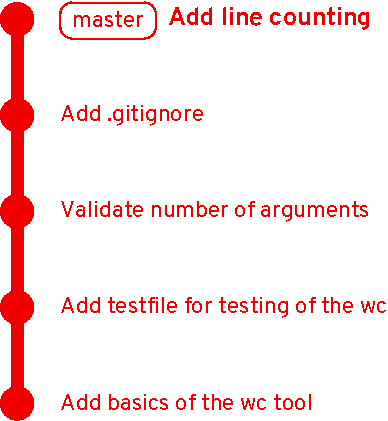
\includegraphics[scale=0.6]{git-figures/02-lines.pdf}
    \hspace{6em}
    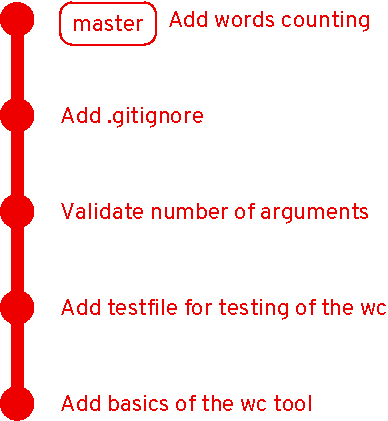
\includegraphics[scale=0.6]{git-figures/02-words.pdf}
  \end{center}
\end{frame}

\begin{frame}
  \frametitle{Basic team synchronisation}
  \vspace{-1em}
  The second one to push must do a merge (and resolve a merge conflict)
  \vspace{1em}
  \begin{center}
    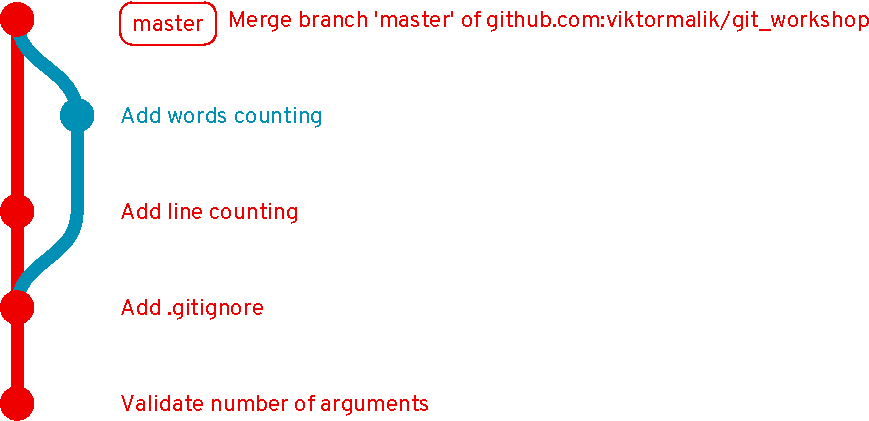
\includegraphics[scale=0.6]{git-figures/02-after-merge.pdf}
  \end{center}
\end{frame}

\begin{frame}
  \frametitle{Better team synchronisation}
  \begin{itemize}
    \setlength\itemsep{.5em}
    \item \textbf{This is not a good practice!}
    \item Always implement new features in \textbf{separate branches}.
    \item Potential merge conflicts should be resolved in the feature branch.
    \item Ideally, merging into master should be always done using \textbf{pull
      requests}
      \begin{itemize}
        \setlength\itemsep{.2em}
        \item They allow other team members to comment on the changes
        \item Changes can be \textbf{reviewed} before they get into master
        \item Master always contains a working and approved version of the
          project
      \end{itemize}
  \end{itemize}
\end{frame}

\begin{frame}[fragile]
  \frametitle{Using a feature branch}
  \vspace{-1em}
  Let us add help into the tool using a separate branch \textit{add\_help}\\
  \begin{verbatim}
  git checkout -b add_help
  git commit -m "Add help for the wc utility"
  \end{verbatim}
  \begin{center}
    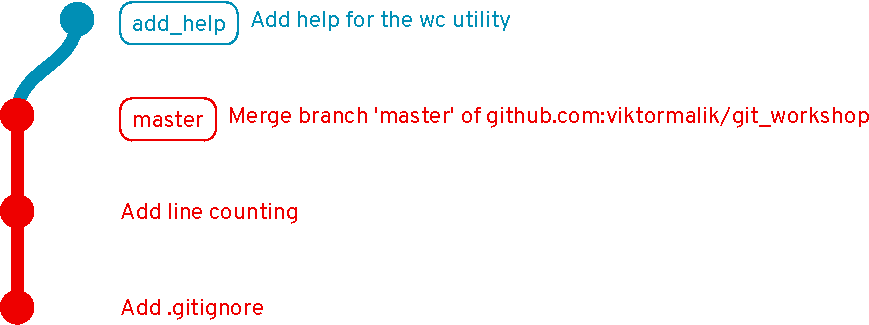
\includegraphics[scale=0.6]{git-figures/03-help.pdf}
  \end{center}
\end{frame}

\begin{frame}
  \frametitle{Using a feature branch}
  \vspace{-1em}
  Then, we open a \textbf{pull request (PR)} from \textit{add\_help} to
  \textit{master}, review it, and merge it using the \textbf{``rebase''}
  strategy.\\[.5em]
  The state of \textit{master} after the PR is merged:
  \vspace{1em}
  \begin{center}
    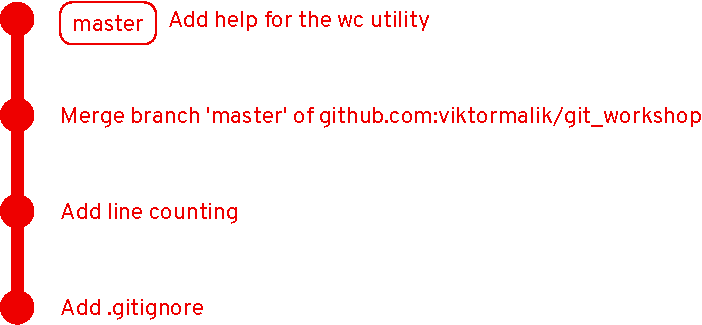
\includegraphics[scale=0.6]{git-figures/03-after-rebase.pdf}
  \end{center}
\end{frame}

\begin{frame}
  \frametitle{Moving branches}
  \vspace{-1em}
  We start working on a new feature (branch \textit{own-separator}) only to
  realize that we need to implement something else before. So, we create
  another branch \textit{option-opt}.\\[.5em]

  But now, we have two branches pointing to the same commit and we need to
  \textbf{move one backwards}.
  \vspace{1em}
  \begin{center}
    \hspace{-2em}
    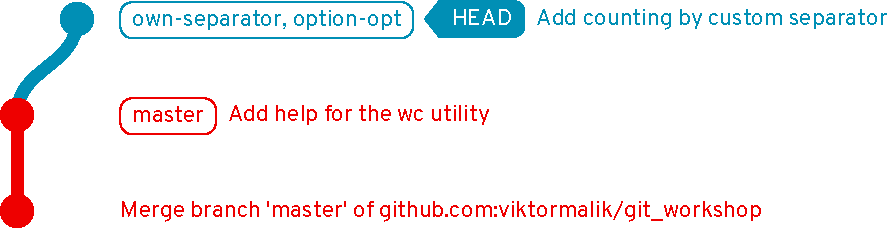
\includegraphics[scale=0.7]{git-figures/04-start.pdf}
  \end{center}
\end{frame}

\begin{frame}[fragile]
  \frametitle{Moving branches}
  \vspace{-1em}
  Instead of deleting and re-creating \textit{option-opt}, we can move it
  \textbf{one commit back}: 
  \begin{verbatim}
  git checkout option-opt
  git reset HEAD^
  \end{verbatim}
  \begin{center}
    \hspace{-2em}
    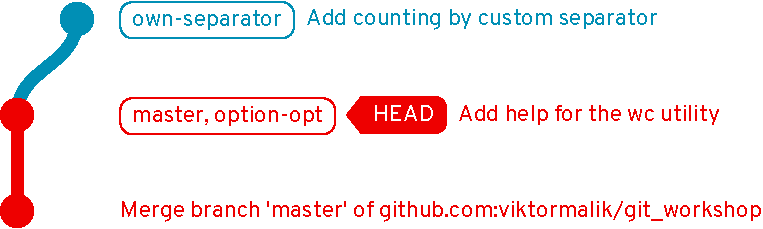
\includegraphics[scale=0.7]{git-figures/04-after-reset.pdf}
  \end{center}
\end{frame}

\begin{frame}
  \frametitle{Moving branches}
  \vspace{-1em}
  After adding a new commit to \textit{options-opt}:
  \vspace{1em}
  \begin{center}
    \hspace{-2em}
    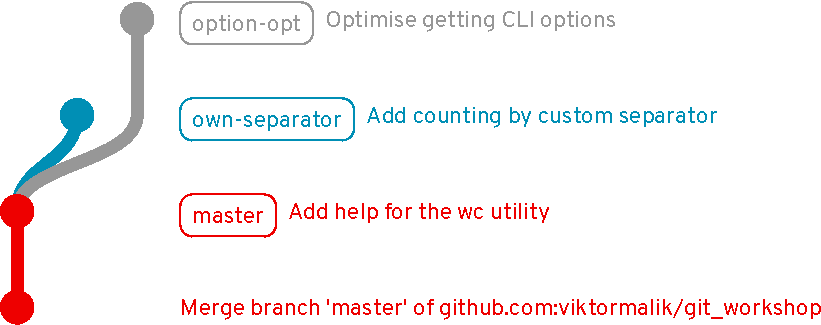
\includegraphics[scale=0.6]{git-figures/04-separate-branches.pdf}
  \end{center}
\end{frame}

\begin{frame}
  \frametitle{Moving branches}
  \vspace{-1em}
  \textit{options-opt} can be now merged into master while
    \textit{own-separator} remains a feature branch in development.
  \vspace{1em}
  \begin{center}
    \hspace{-2em}
    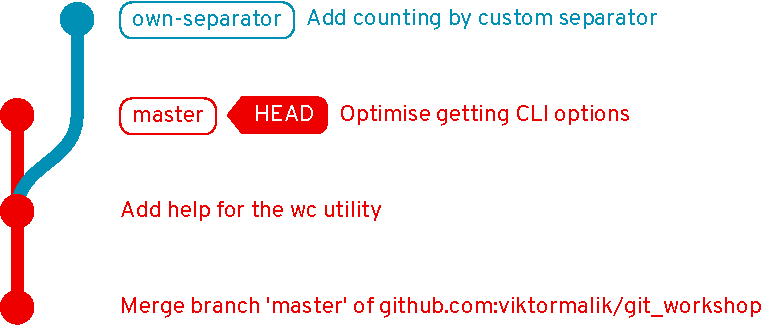
\includegraphics[scale=0.6]{git-figures/04-after-merge.pdf}
  \end{center}
\end{frame}

\begin{frame}[fragile]
  \frametitle{Rebasing feature branches}
  \vspace{-1em}
  We add more commits to the feature branch and then \textbf{rebase} it onto
  \textit{master} (to avoid creation of a merge commit). This introduces a
  \textbf{merge conflict} which we need to resolve using a \textbf{mergetool}
  (we're using \texttt{meld}).
  \begin{verbatim}
  git checkout own-separator
  git commit -m "More robust ..."
  git rebase master
  [... merge conflict ...]
  git mergetool
  \end{verbatim}
  \begin{center}
    \vspace{-7em}
    \hspace{19.5em}
    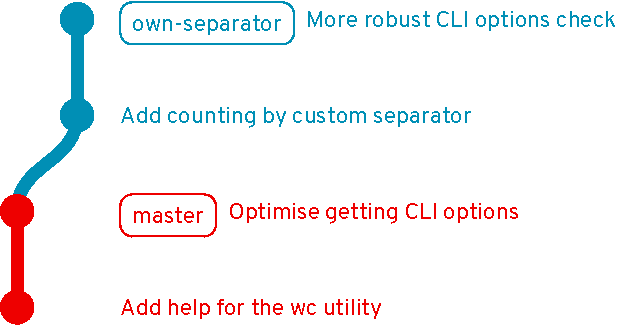
\includegraphics[scale=0.6]{git-figures/04-after-rebase.pdf}
  \end{center}
\end{frame}

\begin{frame}
  \frametitle{Rebasing feature branches}
  \vspace{-1em}
  We made a mistake during the rebase, which we had to fix with an additional
  commit.
  \vspace{1em}
  \begin{center}
    \hspace{-2em}
    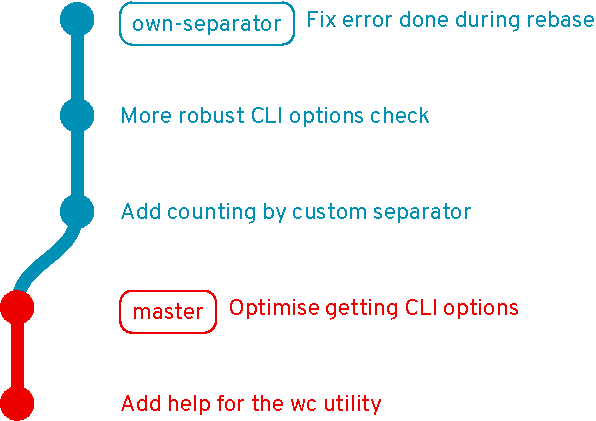
\includegraphics[scale=0.6]{git-figures/04-after-fix.pdf}
  \end{center}
\end{frame}

\begin{frame}[fragile]
  \frametitle{Rebasing feature branches}
  \vspace{-1em}
  It is possible to merge the ``fix commit'' into one of the previous commits
  using \textbf{interactive rebase} (\texttt{git rebase -i master}):\\[.5em]

  Opens up an interactive editor:\\[.3em]
  \small
  \texttt{\textbf{pick} Add counting by custom separator}\\
  \texttt{\textbf{fixup} Fix error done during rebase}\\
  \texttt{\textbf{pick} More robust CLI options check}\\

  \begin{center}
    \vspace{-3em}
    \hspace{21.5em}
    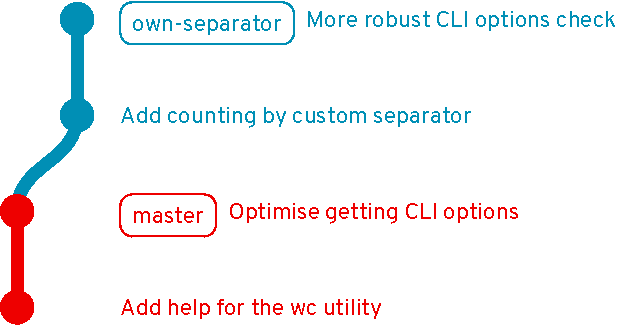
\includegraphics[scale=0.6]{git-figures/04-after-rebase.pdf}
  \end{center}

  \vspace{-7em}
  This merges the second (originally last)\\commit into the first one:
\end{frame}

\begin{frame}
  \frametitle{Interactive rebase}
  \begin{itemize}
    \setlength\itemsep{.5em}
    \item One of the most important Git features in the modern pull
      request-based workflow.
    \item Allows to \textbf{edit}, \textbf{reorder}, \textbf{merge (squash)},
      or \textbf{drop} commits.
    \item \textbf{Rewrites history} -- should be only used on feature branches.
    \item \textbf{Never rewrite history of master!}
      \begin{itemize}
        \item Other developers would not be able to do\, \texttt{git pull}.
      \end{itemize}
  \end{itemize}
\end{frame}

\begin{frame}
  \frametitle{How to rewrite commit history}
  \framesubtitle{Option 1: edit commits via interactive rebase}
  Running interactive rebase and selecting \texttt{edit} for the relevant
  commits:\\[.5em]
  \footnotesize
  \texttt{pick c853f71 unify whitespaces (replace t by 4 spaces)}\\
  \texttt{pick 4fe8acb extend gitignore: added .test-playground}\\
  \texttt{pick 1b7ccf1 Add just comments into the code}\\
  \texttt{\textbf{edit e94003b Improve processing of the cmdline parameters}}\\
  \texttt{pick b5917e8 cmdline parsing: filename is not positional anymore}\\
  \texttt{pick 43b6520 Check the input file has been opened}\\[1em]

  \normalsize
  How to know the right commits? Use \texttt{git blame}.
\end{frame}

\begin{frame}
  \frametitle{How to rewrite commit history}
  \framesubtitle{Option 2: using fixup commits}

  Commit with the \texttt{--fixup} option:\\[.5em]
  \footnotesize
  \texttt{\$ git log --oneline -3}\\
  \texttt{43b6520 Check the input file has been opened}\\
  \texttt{\textbf{b5917e8} cmdline parsing: filename is not positional anymore}\\
  \texttt{\textbf{e94003b} Improve processing of the cmdline parameters}\\
  \texttt{\$ git commit --fixup \textbf{e94003b}}\\
  \texttt{\$ git commit --fixup \textbf{b5917e8}}\\[1em]

  \normalsize
  Now, using interactive rebase with \texttt{--autosquash} will take care of
  everything:\\
  \texttt{git rebase master --interactive \textbf{--autosquash}}
  
\end{frame}

\begin{frame}
  \frametitle{Copying commits from other branches}
  \vspace{-1em}
  It is possible to \textbf{copy commits} from other branches (e.g. commits
  implementing useful features from co-workers feature branches) using\,
  \texttt{git cherry-pick}.\\
  \vspace{1em}
  The \textit{recursion} branch:
  \begin{center}
    \vspace{-1.5em}
    \hspace{7em}
    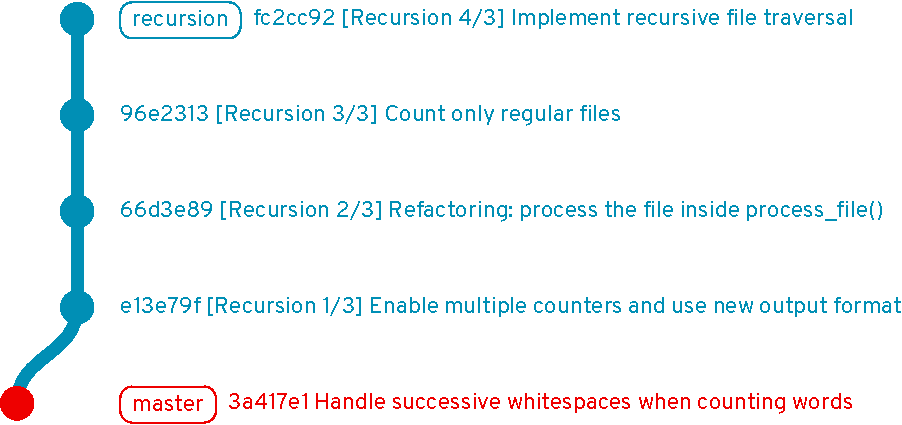
\includegraphics[scale=0.6]{git-figures/05-recursion.pdf}
  \end{center}
\end{frame}

\begin{frame}[fragile]
  \frametitle{Copying commits from other branches}
  \vspace{-1em}
  Now, let's create a new branch \textit{multiple-files}, cherry-pick the first
  three commits from \textit{recursion}, and add a new commit on top:
  \footnotesize
  \begin{verbatim}
git checkout -b multiple-files
git cherry-pick e13e79f^..96e2313
git commit -m "Support ..."
  \end{verbatim}

  \normalsize
  Equivalent cherry-pick range:\\
  \small
  \texttt{recursion@\{4\}..recursion@\{1\}}

  \begin{center}
    \vspace{-9.5em}
    \hspace*{18em}
    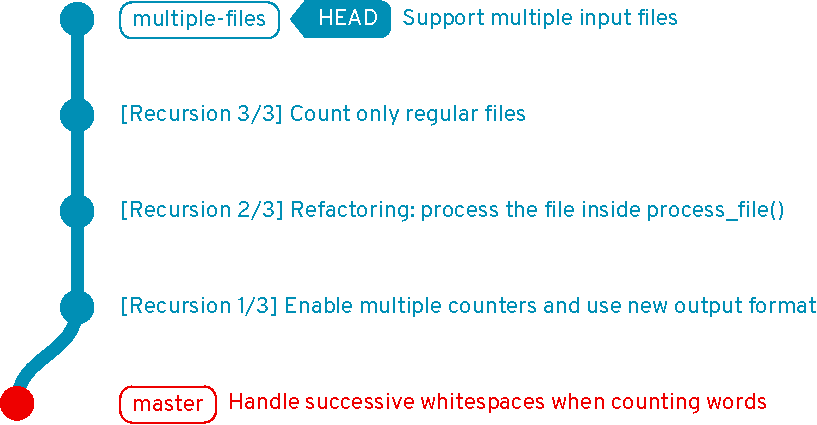
\includegraphics[scale=0.6]{git-figures/05-multiple-files.pdf}
  \end{center}

\end{frame}

\begin{frame}
  \frametitle{Copying commits from other branches}
  \vspace{-1.5em}
  \small
  Finally, we rewrite the cherry-picked commits:\\[.3em]
  \footnotesize
  \texttt{\textbf{edit} 9abab39 [Recursion 1/3] Enable multiple counters and
    use new ...}\\
  \texttt{\textbf{reword} 2c403cc [Recursion 2/3] Refactoring: process the file
    inside ...}\\
  \texttt{\textbf{reword} f85bb09 [Recursion 3/3] Count only regular files}\\
  \texttt{pick Support multiple input files}\\[1em]

  \small
  Then, we try to rebase \texttt{recursion} on top of
  \texttt{multiple-files}:\\[.3em]
  \footnotesize
  \texttt{git checkout recursion}\\
  \texttt{git rebase multiple-files}\\
  \texttt{[... \textbf{merge conflict during applying [Recursion 1/3]}
    ...]}\\[1em]
  \small
  Git tried to apply the first commit from \textit{recursion}
  (\texttt{e13e79f}) but the commit is already in
  \textit{multiple-files}. Git failed to recognise that since we altered the
  commit.

  The solution is to use \texttt{\textbf{git rebase --skip}} for such commits.
  %\begin{center}
    %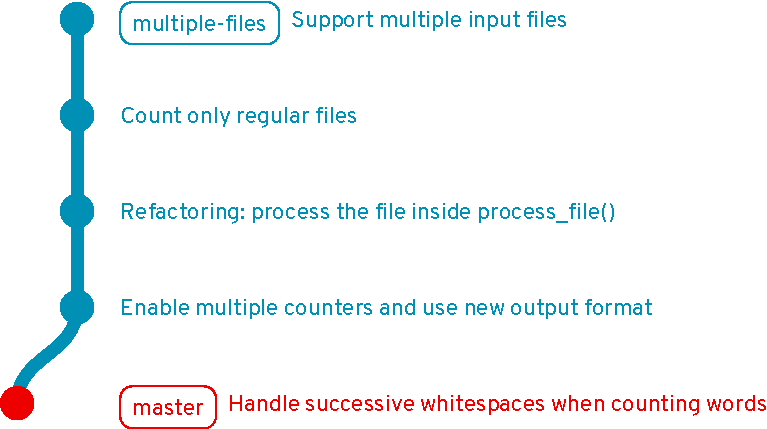
\includegraphics[scale=0.6]{git-figures/05-multiple-files-rebase.pdf}
  %\end{center}
\end{frame}

\begin{frame}
  \frametitle{Hunting bugs in Git history}
  \vspace{-1em}
  \begin{itemize}
    \setlength\itemsep{.5em}
    \item We often discover a bug that was certainly introduced
      \textbf{somewhere in the Git history}.
      \begin{itemize}
        \item There is a revision in the past where certain test works correctly.
        \item However, the test does not work now.
      \end{itemize}
    \pause
    \item Git offers \texttt{git bisect} that uses \textbf{binary search} to
      localise the commit that caused the bug.
      \begin{itemize}
        \item \texttt{git bisect start }starts bisecting.
        \item \texttt{git bisect good }marks a commit that does not contain
          the bug.
        \item \texttt{git bisect bad }marks a commit contains the bug.
        \item \texttt{git bisect skip }marks a commit that cannot be evaluated.
      \end{itemize}
    \pause
    \item The process can be \textbf{automated} using a script that returns 0
      on success and a non-zero result on failure.
  \end{itemize}
\end{frame}

\section{Git tips and tricks}

\begin{frame}
  \frametitle{Cloning repositories with a long history}
  \begin{itemize}
    \setlength\itemsep{.5em}
    \item If a repo has a long history, it may take long time to clone it.
    \item If the entire history is no needed, it is possible to use a
      \textbf{shallow copy}:\\ \texttt{git clone --max-depth N}
    \item Try it with the Linux kernel:\\
      \texttt{git clone --max-depth 1 https://github.com/torvalds/linux}
  \end{itemize}
\end{frame}

\begin{frame}
  \frametitle{Signing commits}
  \begin{itemize}
    \setlength\itemsep{.5em}
    \item By default, it is not possible to verify that a certain commit was
      truly created by the person who is stated as the author.
    \item Theoretically, anyone can set your name and email as theirs and
      commit on your behalf.
    \pause
    \item To resolve this problem, Git offers \textbf{signing commits} using
      GPG keys.
    \item GitHub offers a nice tutorial on how to setup commit signing:
      \url{https://help.github.com/en/github/authenticating-to-github/signing-commits}
  \end{itemize}
\end{frame}

\begin{frame}
  \frametitle{Setup your environment}
  \vspace{-2em}
  There are various possibilities on how to ease your life with Git:
  \begin{itemize}
    \setlength\itemsep{.5em}
    \item \textbf{Git prompt}
      \begin{itemize}
        \item It is possible to setup Bash prompt such that it shows the
          current branch, state of the directory, etc.
        \item There are many tutorials on how to set the prompt
        \item Some alternative shells (e.g. Fish, zsh) include Git prompt by
          default
      \end{itemize}
    \pause
    \item \textbf{IDE/Editor support}
      \begin{itemize}
        \item It is useful to see which lines were added/removed/changed from
          HEAD.
        \item Most IDEs and editors offer a way to setup this.
      \end{itemize}
    \pause
    \item \textbf{Use tools for history inspection}
      \begin{itemize}
        \item There is a number of tools for an easier history traversal
        \item E.g. \textbf{tig}, gitk, \ldots
      \end{itemize}
  \end{itemize}
\end{frame}

\begin{frame}
  \frametitle{Git and IDEs/Editors}
  \vspace{-2em}
  Overcome The Doorway Effect of switching to your terminal, examples:
  \pause
  \begin{itemize}
    \setlength\itemsep{.5em}
    \item \textbf{VSCode}
      \begin{itemize}
         \item Highlight added/changed/removed lines
         \item Git blame for each line
         \item Commit, push, pull etc.
      \end{itemize}
    \pause
    \item \textbf{Vim}
      \begin{itemize}
	\item \textbf{git-gutter}
	  \begin{itemize}
	     \item Display line status on the side
	  \end{itemize}
        \item \textbf{vim-fugitive}
	  \begin{itemize}
	     \item Full fledged TUI for Git right in your Vim
	     \item Commit, push, pull etc.
	     \item \texttt{<Esc>:G-cciExample commit<Esc>:x-}
	  \end{itemize}
      \end{itemize}
  \end{itemize}
\end{frame}

\begin{frame}[fragile]
  \frametitle{Setup your environment}
  \vspace{-1em}
  \begin{itemize}
    \setlength\itemsep{.5em}
    \item \textbf{Command aliases}
      \begin{itemize}
        \setlength\itemsep{.5em}
        \item Many Git commands are quite long (or have many options).
        \item It is possible to setup short aliases for most commonly used
          commands.
        \item Git offers a way to set aliases:\\
          \texttt{git config --global alias.co checkout\\...}\\
          or edit \texttt{\$HOME/.gitconfig}:\\
          \texttt{
            [alias]\\
            \quad co = checkout\\
            \quad ...}
        \item An alternative is to setup aliases via shell
      \end{itemize}
  \end{itemize}
\end{frame}

\begin{frame}
  \frametitle{Keep your repo clean}
  \begin{itemize}
    \item Delete merged/obsolete branches (locally)
      \begin{itemize}
        \item \texttt{git branch -d }doesn't always work (especially with
          rebases)
        \item \texttt{git branch -D }works but be careful not to delete
          something important
      \end{itemize}
    \vspace{.5em}
    \item Same applies for remote branches
      \begin{itemize}
        \item \texttt{git push --delete <remote> <branch>}
        \item or enable auto-delete branch on your PRs
        \item or use GitHub/GitLab/\ldots web UI
      \end{itemize}
    \vspace{.5em}
    \item \texttt{git prune }removes unreachable objects (branches, tags, etc.)
  \end{itemize}
\end{frame}

\begin{frame}
  \frametitle{Other interesting git commands}
  \begin{itemize}
    \item \texttt{git difftool} -- open mergetool for a specific commit and
      file
    \item \texttt{git worktree} -- checkout a branch into a directory
    \item \texttt{git submodule} -- embed another git repository
    \item \texttt{git grep} -- grep the entire repository
    \item \texttt{git describe} -- find tags related to commit
    \item \texttt{git reflog} -- the last recovery option when you break your
      repo
  \end{itemize}
\end{frame}

\begin{frame}
  \frametitle{Useful links}
  \begin{itemize}
    \item Atlassian Advanced Git Tutorials\\
      \url{https://www.atlassian.com/git/tutorials/advanced-overview}
    \item GitHub Guides\\
      \url{https://guides.github.com}
    \item GitHub Help\\
      \url{https://help.github.com/en/github}
  \end{itemize}
\end{frame}

\begin{frame}
  \frametitle{TL;DR}
  What you should take out of this talk:
  \begin{itemize}
    \item Learn and practice \textbf{interactive rebase}
    \item \textbf{Read what Git tells you}, there are often good hints (e.g.
      for undoing things)
    \item Keep \textit{master} in good shape
  \end{itemize}
  \setbeamerfont{thankyou}{size=\fontsize{19pt}{2pt}}
  \vspace*{2em}
  \centering
  {\usebeamerfont{thankyou}\hl{Thank you for the attention!}}\\[1em]
  Your feedback is welcome!\\\texttt{https://forms.gle/2D4LfsYz5MGjDfWL7}
\end{frame}

\end{document}
